\documentclass[11pt, a4paper, openany]{book}
\usepackage{graphicx}
\usepackage{colortbl}
\usepackage{amsmath}
\usepackage{tikz}
\usepackage{blindtext}
\usepackage{microtype}
\usepackage{wrapfig}
\usepackage{enumitem}
\usepackage{fancyhdr}
\usepackage{index}
\usepackage{tcolorbox}
\usepackage{booktabs}
\usepackage[margin=1in]{geometry}
\usepackage[english]{babel}
%\usepackage{times}

\makeindex
\title{\textbf{IGCSE Economics Subject Content 1}}
\author{Ang Li, Frank}
\date{May 26, 2019}
\usetikzlibrary{decorations.pathreplacing}

\begin{document}

\pagenumbering{roman}
\newcommand{\head}[1]{\textnormal{\textbf{#1}}}

\fancyhf{}
\renewcommand{\headrulewidth}{2pt}
\renewcommand{\footrulewidth}{1pt}
\fancyhead[LE]{\leftmark}
\fancyhead[RO]{\nouppercase{\rightmark}}
\fancyfoot[LE, RO]{\thepage}

\maketitle
\tableofcontents

\chapter{The Basic Economic Problem}

\begin{tcolorbox}
\textbf{Key points from this section:}
\begin{enumerate}\itemsep0em
	\item Define the nature of the economic problem.
	\item Define the factors of production.
	\item Define opportunity cost and illustration of the concept.
	\item Demonstrate how production possibility curves can be used to illustrate choice and resource allocation.
	\item Evaluate the implications of particular courses of action in terms of opportunity cost.
\end{enumerate}
\end{tcolorbox}

\section{The Nature of the Economic Problem}

\subsection{Finite resources and unlimited wants}

\begin{itemize}\itemsep0em
	\item \textbf{The basic economic problem:} How to allocate scarce resources to satisfy unlimited needs and wants.
	\item \textbf{Scarcity:} Unlimited wants and not enough resources to fulfill the wants.
	\item \textbf{Unlimited wants:} The unlimited desires that people have.
	\item \textbf{Limited resources:} The limited factors of production (resources) that we have on Earth.
    \item \textbf{Needs:} Things which we require in order to survive.
    \item \textbf{Wants:} Things that we do not need but want for enjoyment or utility.
    \item \textbf{Basic economic questions:}
        \begin{enumerate}\itemsep0em
            \item What to product.
            \item How to produce it.
            \item For whom to produce it.
        \end{enumerate}
\end{itemize}

\subsection{Economic and free goods}

\begin{itemize}\itemsep0em
    \item \textbf{Goods:} Physical items, e.g. books, computers, and food.
    \item \textbf{Services:} Non-physical items, e.g. haircuts and internet access.
    \item \textbf{Economic goods:} Goods that are limited in supply, e.g. cars, paper, and oil.
    \item \textbf{Free goods:} Goods that are unlimited in suppy, e.g. air, sea, and public web pages.
    \item \textbf{Economic agents:} Individuals, firms, and the government.
\end{itemize}

\section{The Factors of Production}

\subsection{Definitions of the factors of production and their rewards}

\begin{itemize}\itemsep0em
    \item \textbf{Four factors of production (LLCE):}
        \begin{enumerate}\itemsep0em
            \item \textbf{Land:} The natural resources required in a production process, e.g. wood and oil.
            \item \textbf{Labor:} The human resources required in a production (physical or mental, skilled or unskilled), e.g. teacher and police.
            \item \textbf{Capital:} The manufactured resources required in a production, e.g. machinery and tools.
            \item \textbf{Enterprise:} The skills in a business person requires to manage the other three factors of production and the ability to undertake risks.
        \end{enumerate}
    \item \textbf{Four rewards to factors of production (RWIP):}
        \begin{enumerate}\itemsep0em
            \item \textbf{Rent:} Reward or payment for \textit{land} resources.
            \item \textbf{Wage/Salary:} Reward or payment for \textit{labor} resources.
            \item \textbf{Interest:} Reward or payment for \textit{capital} resources.
            \item \textbf{Profit:} Reward or payment for \textit{enterprise} resources.
        \end{enumerate}
\end{itemize}

\subsection{Mobility of the factors of production}

\begin{itemize}\itemsep0em
    \item \textbf{Geographical mobility:} The ability of factors of production (except land) to move around an area, region or country in order to work.
    \item \textbf{Horizontal mobility:} The ability of factors of production (mostly labor) to move from one occupation to another with the same social level.
    \item \textbf{Occupational mobility:} The ability of factors of production (mostly labor) to swtich career fields.
\end{itemize}\itemsep0em

%\subsection{Quantity and quality of the factors of production}
%
%\begin{itemize}\itemsep0em
%    \item \textbf{Factors affecting the quatity of the factors of production:}
%        \begin{enumerate}\itemsep0em
%            \item
%        \end{enumerate}
%    \item \textbf{Factors affecting the quality of the factors of production:}
%        \begin{enumerate}\itemsep0em
%            \item
%        \end{enumerate}
%\end{itemize}

\section{Opportunity Cost}

\subsection{Definition of opportunity cost}

\begin{itemize}\itemsep0em
    \item \textbf{Opportunity cost:} The next best alternative given up when making a decision. (Doesn't have to be money)
        \begin{itemize}\itemsep0em
            \item The opportunity cost of taking economics course is the other subject you would be studying instead.
            \item The opportunity cost of playing games is the other things that you could be instead like studying.
            \item The opportunity cost of funding the military could be free or well-funded healthcare.
        \end{itemize}
\end{itemize}

\subsection{The influence of opportunity cost on decision making}

\begin{itemize}\itemsep0em
    \item \textbf{Consumers:} Purchasing one good causes opportunity cost of the other good.
    \item \textbf{Producers:} Producing one good causes opportunity cost of the other good.
    \item \textbf{Government:} Passing one policy causes opportunity cost of the other policy.
\end{itemize}

\section{Production Possibility Curve Diagrams (PPC)}

\subsection{Definition of PPC}

\begin{itemize}\itemsep0em
    \item \textbf{Production possibility curve:} A graph illustrating the production of two goods, used to display opportunity cost.
    \item It is a graph with the number of production of two goods as the two axies, where the two goods share a certain factor of
        production to produce. Thus, resulting in a downward sloping curve.
    \item \textbf{Two types of PPC}
        \begin{figure}[!h]
            \centering
            \begin{minipage}{0.45\textwidth}
                \begin{tikzpicture}[scale=1]
                    \draw (0,5) node [left] {$Y$} -- (0,0) node [below left] {$0$} -- (5.5,0) node [below] {$X$};
                    \draw (0,4.1) to [out=-5, in=140] (2.8,3.1) to [out=-40, in=105] (4.8,0);
                \end{tikzpicture}
                \caption{PPC with specialization}
            \end{minipage}
            \hspace{0.3cm}
            \begin{minipage}{0.45\textwidth}
                \begin{tikzpicture}[scale=1]
                    \draw (0,5) node [left] {$Y$} -- (0,0) node [below left] {$0$} -- (5.5,0) node [below] {$X$};
                    \draw (0,4.1) -- (4.8,0);
                \end{tikzpicture}
                \caption{PPC without specialization}
            \end{minipage}
        \end{figure}
        \begin{itemize}\itemsep0em
            \item \textit{Figure 1.1:} Increasing opportunity cost due to specialization. (Resources required are not the same)
            \item \textit{Figure 1.2:} Constant opportunity cost due to no specialization. (Resources required are identical)
        \end{itemize}
\end{itemize}

\subsection{Points under, on, and beyond a PPC}

\vspace{-0.3cm}
\begin{figure}[!h]
    \begin{minipage}{0.45\textwidth}
        \textbf{Keys:}
        \begin{itemize}[leftmargin=*]\itemsep0em
%            \item \textbf{Y-axis} The number of production of good Y.
%            \item \textbf{X-axis} The number of production of good X
            \item \textit{Point A:} All resources dedicated to the production of good Y.
            \item \textit{Point B:} All resources dedicated to the production of good X.
            \item \textit{Point C:} $X_1$ amount of good X produced along with $Y_1$ amount of good Y.
            \item \textit{Point D:} $X_2$ amount of good X produced along with $Y_2$ amount of good Y.
            \item \textit{Point E:} Resources are not allocated at the maximum efficiency.
            \item \textit{Point F:} This point of production is unattainable. (Not enough resources)
        \end{itemize}
    \end{minipage}
    \hspace{0.3cm}
    \begin{minipage}{0.3\textwidth}
        \begin{tikzpicture}[scale=1.2]
            \draw (0,5) node [left] {$Y$} -- (0,0) node [below left] {$0$} -- (5.5,0) node [below] {$X$};
            \draw (0,4.1) to [out=-5, in=140] (2.8,3.1) to [out=-40, in=105] (4.8,0);
            \node [left] at (0,4.1) {$A$};
            \draw [fill] (0,4.1) circle [radius=.05];
            \node [above left] at (4.7,0) {$B$};
            \draw [fill] (4.8,0) circle [radius=.05];
            \node [above right] at (2.7,3.2) {$C$};
            \draw [fill] (2.7,3.2) circle [radius=.05];
            \node [above] at (4.1,2) {$D$};
            \draw [fill] (3.9,2) circle [radius=.05];
            \draw [dashed] (0,3.2) -- (2.7,3.2);
            \node [left] at (0,3.2) {$Y_1$};
            \draw [fill] (0,3.2) circle [radius=.05];
            \draw [dashed] (0,2) -- (3.9,2);
            \node [left] at (0,2) {$Y_2$};
            \draw [fill] (0,2) circle [radius=.05];
            \draw [dashed] (2.7,3.2) -- (2.7,0);
            \node [left] at (3,-0.3) {$X_1$};
            \draw [fill] (2.7,0) circle [radius=.05];
            \draw [dashed] (3.9,2) -- (3.9,0);
            \node [left] at (4.2,-0.3) {$X_2$};
            \draw [fill] (3.9,0) circle [radius=.05];
            \node [left] at (2,1.6) {$E$};
            \draw [fill] (2,1.6) circle [radius=.05];
            \node [left] at (4,4) {$F$};
            \draw [fill] (4.2,4) circle [radius=.05];
        \end{tikzpicture}
    \end{minipage}
    \caption{Generic PPC graph with points}
\end{figure}

\subsection{Movements along a PPC}

\begin{itemize}\itemsep0em
    \item \textbf{Movement along a PPC:} This happens when the producer alters its production.
    \item For example, originally a company was producing at \textit{Point C}, which is $X_1$ amount of good X
        and $Y_1$ amount of good Y.(\textit{Figure 1.4}) In this case the opportunity cost will be the amount of good Y
        that was not produced, which is $OC_1$ $(A - Y_1)$.
    \item After a while the company decides to change its production and produce at \textit{Point D} $(X_2, Y_2)$, this decision's
        opportunity cost would be $OC_2$ $(Y_1 - Y_2)$ as the amount given up by this specific decision is $Y_1 - Y_2$.
    \item This is a movement along the PPC from \textit{Point C} to \textit{Point D}.
        \begin{figure}[!h]
            \centering
            \begin{minipage}{0.45\textwidth}
                \begin{tikzpicture}[scale=1]
                    \draw (0,5) node [left] {$Y$} -- (0,0) node [below left] {$0$} -- (5.5,0) node [below] {$X$};
                    \draw (0,4.1) to [out=-5, in=140] (2.8,3.1) to [out=-40, in=105] (4.8,0);
                    \node [left] at (0,4.1) {$A$};
                    \draw [fill] (0,4.1) circle [radius=.05];
                    \node [above left] at (4.7,0) {$B$};
                    \draw [fill] (4.8,0) circle [radius=.05];
                    \node [above right] at (2.7,3.2) {$C$};
                    \draw [fill] (2.7,3.2) circle [radius=.05];
                    \node [above] at (4.1,2) {$D$};
                    \draw [fill] (3.9,2) circle [radius=.05];
                    \draw (0,3.2) -- (2.7,3.2);
                    \node [left] at (0,3.2) {$Y_1$};
                    \draw [fill] (0,3.2) circle [radius=.05];
                    \draw [dashed] (0,2) -- (3.9,2);
                    \node [left] at (0,2) {$Y_2$};
                    \draw [fill] (0,2) circle [radius=.05];
                    \draw (2.7,3.2) -- (2.7,0);
                    \node [left] at (3,-0.3) {$X_1$};
                    \draw [fill] (2.7,0) circle [radius=.05];
                    \draw [dashed] (3.9,2) -- (3.9,0);
                    \node [left] at (4.2,-0.3) {$X_2$};
                    \draw [fill] (3.9,0) circle [radius=.05];
                    \draw [decorate,decoration={brace,amplitude=5pt,mirror,raise=4pt},yshift=0pt] (0,3.2) -- (0,4.1)
                        node [black,midway,xshift=0.7cm]{\footnotesize$OC_1$};
                \end{tikzpicture}
                \caption{Before}
            \end{minipage}
            \hspace{0.3cm}
            \begin{minipage}{0.45\textwidth}
                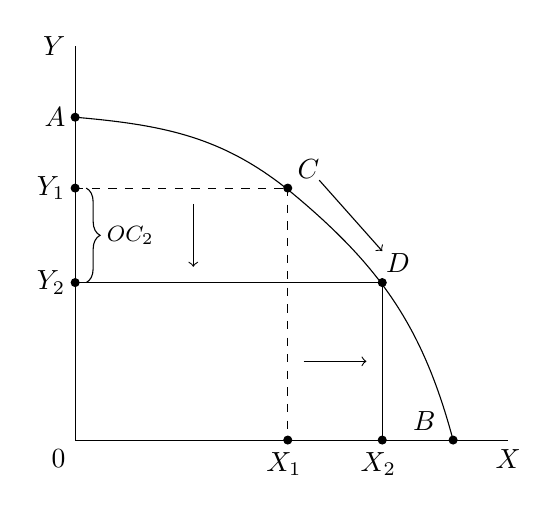
\begin{tikzpicture}[scale=1]
                    \draw (0,5) node [left] {$Y$} -- (0,0) node [below left] {$0$} -- (5.5,0) node [below] {$X$};
                    \draw (0,4.1) to [out=-5, in=140] (2.8,3.1) to [out=-40, in=105] (4.8,0);
                    \node [left] at (0,4.1) {$A$};
                    \draw [fill] (0,4.1) circle [radius=.05];
                    \node [above left] at (4.7,0) {$B$};
                    \draw [fill] (4.8,0) circle [radius=.05];
                    \node [above right] at (2.7,3.2) {$C$};
                    \draw [fill] (2.7,3.2) circle [radius=.05];
                    \node [above] at (4.1,2) {$D$};
                    \draw [fill] (3.9,2) circle [radius=.05];
                    \draw [dashed] (0,3.2) -- (2.7,3.2);
                    \node [left] at (0,3.2) {$Y_1$};
                    \draw [fill] (0,3.2) circle [radius=.05];
                    \draw (0,2) -- (3.9,2);
                    \node [left] at (0,2) {$Y_2$};
                    \draw [fill] (0,2) circle [radius=.05];
                    \draw [dashed] (2.7,3.2) -- (2.7,0);
                    \node [left] at (3,-0.3) {$X_1$};
                    \draw [fill] (2.7,0) circle [radius=.05];
                    \draw (3.9,2) -- (3.9,0);
                    \node [left] at (4.2,-0.3) {$X_2$};
                    \draw [fill] (3.9,0) circle [radius=.05];
                    \draw [decorate,decoration={brace,amplitude=5pt,mirror,raise=4pt},yshift=0pt] (0,2) -- (0,3.2)
                        node [black,midway,xshift=0.7cm]{\footnotesize$OC_2$};
                    \draw [->] (1.5,3) -- (1.5,2.2);
                    \draw [->] (2.9,1) -- (3.7,1);
                    \draw [->] (3.1,3.3) -- (3.9,2.4);
                \end{tikzpicture}
                \caption{After}
            \end{minipage}
        \end{figure}
\end{itemize}

\subsection{Shifts in a PPC}

<++>

\end{document}
